\documentclass[12pt]{report}
\usepackage[spanish]{babel}
\usepackage[utf8]{inputenc}
\usepackage{amsmath}
\usepackage{amssymb}
\usepackage{amsthm}
\usepackage{graphics}
\usepackage{subfigure}
\usepackage{lipsum}
\usepackage{array}
\usepackage{multicol}
\usepackage{enumerate}
\usepackage[framemethod=TikZ]{mdframed}
\usepackage[a4paper, margin = 1.5cm]{geometry}
\usepackage{wrapfig}

%En esta parte se hacen redefiniciones de algunos comandos para que resulte agradable el verlos%

\renewcommand{\theenumii}{\roman{enumii}}

\def\proof{\paragraph{Demostración:\\}}
\def\endproof{\hfill$\blacksquare$}

\def\sol{\paragraph{Solución:\\}}
\def\endsol{\hfill$\square$}

%En esta parte se definen los comandos a usar dentro del documento para enlistar%

\newtheoremstyle{largebreak}
  {}% use the default space above
  {}% use the default space below
  {\normalfont}% body font
  {}% indent (0pt)
  {\bfseries}% header font
  {}% punctuation
  {\newline}% break after header
  {}% header spec

\theoremstyle{largebreak}

\newmdtheoremenv[
    leftmargin=0em,
    rightmargin=0em,
    innertopmargin=0pt,
    innerbottommargin=5pt,
    hidealllines = true,
    roundcorner = 5pt,
    backgroundcolor = gray!60!red!30
]{exa}{Ejemplo}[section]

\newmdtheoremenv[
    leftmargin=0em,
    rightmargin=0em,
    innertopmargin=0pt,
    innerbottommargin=5pt,
    hidealllines = true,
    roundcorner = 5pt,
    backgroundcolor = gray!50!blue!30
]{obs}{Observación}[section]

\newmdtheoremenv[
    leftmargin=0em,
    rightmargin=0em,
    innertopmargin=0pt,
    innerbottommargin=5pt,
    rightline = false,
    leftline = false
]{theor}{Teorema}[section]

\newmdtheoremenv[
    leftmargin=0em,
    rightmargin=0em,
    innertopmargin=0pt,
    innerbottommargin=5pt,
    rightline = false,
    leftline = false
]{propo}{Proposición}[section]

\newmdtheoremenv[
    leftmargin=0em,
    rightmargin=0em,
    innertopmargin=0pt,
    innerbottommargin=5pt,
    rightline = false,
    leftline = false
]{cor}{Corolario}[section]

\newmdtheoremenv[
    leftmargin=0em,
    rightmargin=0em,
    innertopmargin=0pt,
    innerbottommargin=5pt,
    rightline = false,
    leftline = false
]{lema}{Lema}[section]

\newmdtheoremenv[
    leftmargin=0em,
    rightmargin=0em,
    innertopmargin=0pt,
    innerbottommargin=5pt,
    roundcorner=5pt,
    backgroundcolor = gray!30,
    hidealllines = true
]{mydef}{Definición}[section]

\newmdtheoremenv[
    leftmargin=0em,
    rightmargin=0em,
    innertopmargin=0pt,
    innerbottommargin=5pt,
    roundcorner=5pt
]{excer}{Ejercicio}[section]
%En esta parte se colocan comandos que definen la forma en la que se van a escribir ciertas funciones%

\newcommand\abs[1]{\ensuremath{\lvert#1\rvert}}
\newcommand\divides{\ensuremath{\bigm|}}
\newcommand\aut{\textup{Aut}}
\newcommand\irr{\textup{irr}}

%recuerda usar \clearpage para hacer un salto de página

\begin{document}
    \setlength{\parskip}{5pt} % Añade 5 puntos de espacio entre párrafos
    \setlength{\parindent}{12pt} % Pone la sangría como me gusta
    \title{Lista Extensiones Normales AM III}
    \author{Cristo Daniel Alvarado}
    \date{Diciembre de 2023}
    \maketitle

\setcounter{chapter}{2}

\chapter{Ejercicios}

\section{Extensiones Normales}

\begin{excer}
    Sea $E/F$ una extensión de campos. Denotamos por $\textup{Aut}(E)$ (resp. $\textup{Aut}_F(E)$) al conjunto de todos los automorfismos (resp. $F$-automorfismos) de $E$. Demuestre que $\textup{Aut}(E)$ es un grupo con la compsición de funciones, y que $\textup{Aut}_F(E)$ es un subgrupo de $\textup{Aut}(E)$.
\end{excer}

\begin{proof}
    Claramente el resultado se tiene de que $\textup{Aut}(E)$ es un grupo con la composición de funciones. Veamos que $\textup{Aut}_F(E)$ es un subgrupo. En efecto, el conjunto $\textup{Aut}_F(E)$ es no vacío pues $\textup{id}_E\in\textup{Aut}_F(E)$. Ahora, sean $f,g\in\textup{Aut}(E)$, se tiene que
    \begin{equation}
        f(\alpha)=\alpha=g(\alpha),\quad\forall \alpha\in F.
    \end{equation}
    donde $f,g\in \textup{Aut}(E)$. En particular, se tiene que $f\circ g^{-1}$ es un elemento de $\textup{Aut}(E)$. Y además:
    \begin{equation}
        \begin{split}
            g^{-1}(\alpha)=&g^{-1}(g(\alpha))\\
            =&\alpha,\quad \forall\alpha\in F\\
        \end{split}
    \end{equation}
    es decir, $g^{-1}$ es un $F$-automorfismo de $E$. Por tanto
    \begin{equation}
        \begin{split}
            f\circ g^{-1}(\alpha)=&f(g^{-1}(\alpha))\\
            =&f(\alpha)\\
            =&\alpha,\quad \forall \alpha\in F\\
        \end{split}
    \end{equation}
    entonces, $f\circ g^{-1}\in \textup{Aut}_F(E)$. Luego, $\textup{Aut}_F(E)<\textup{Aut}(E)$.
\end{proof}

\begin{excer}
    Calcule $\aut_{\mathbb{R}}(\mathbb{Q})$ y $\aut_{K}(K(X))$ donde $K(X)$ es el campo de funciones racionales en la variable $X$ sobre $K$.
\end{excer}

\begin{proof}
    
\end{proof}

\begin{excer}
    Sea $E$ el campo de descomposición de un polinomio $f(X)\in F[X]$ con $\deg(f)=n\geq1$, donde $E/F$ es extensión de campos. Pruebe que $[E:F]$ divide a $n!$. Más aún, el grupo $\textup{Aut}_F(E)$ está encajado en el grupo simétrico $S_n$ de grado $n$.
\end{excer}

\begin{proof}
    Como $E$ es el campo de descomposición de $f(X)$, entonces expresamos a $E=F\left(u_1,\dots,u_n\right)$, donde $u_1,\dots,u_n\in E$ son las raíces del polinomio $f(X)$.
\end{proof}

\begin{excer}
    Sean $\alpha, \beta$ algebraicos sobre $F$, y sean $f(X)=\irr(\alpha, F, X)$ y $g(X)=\irr(\beta, F, X)$ tales que $\deg(f)$ y $\deg(g)$ son primos relativos. Demuestre que $g$ es irreducible sobre $F(\alpha)[X]$.
\end{excer}

\begin{proof}
    Por un ejercicio de la lista anterior, se tiene que
    \begin{equation*}
        [F(\alpha,\beta):F(\alpha)]=[F(\beta):F]
    \end{equation*}
    por ser $\deg(f)$ y $\deg(g)$ primos relativos (en realidad, se tiene que $[F(\alpha,\beta):F]=[F(\alpha):F][F(\beta):F]$, esto implica la igualdad de arriba). Por tanto, si $g$ no fuera irreducible sobre $F(\alpha)$, se tendría que
    \begin{equation*}
        [F(\alpha,\beta):F(\alpha)]=[F(\alpha)(\beta):F(\alpha)]<[F(\beta):F]
    \end{equation*}
    pues, en este caso se tendría que $h(X)=\irr(\beta,F(\alpha),X)|g(X)$, con $\deg(h)<\deg(g)$, lo cual contradice la ecuación anterior. Por tanto, $g$ es irredicible sobre $F(\alpha)$.
\end{proof}

\begin{excer}
    Sea $\alpha$ una raíz del polinomio $X^6+X^3+1$ sobre $\mathbb{Q}$. Encunetre todos los homomorfismos de $\mathbb{Q}(\alpha)$ en $\mathbb{C}$.(Sugerencia: El polinomio es factor del polinomio $X^9-1$).
\end{excer}

\begin{proof}
    
\end{proof}

\begin{excer}
    Encunetre el campo de descomposición de los siguientes polinmoios sobre $\mathbb{Q}$, y el grado de tales campos de descomposición sobre $\mathbb{Q}$.
    \begin{enumerate}
        \item $X^3-2$.
        \item $X^2+X+1$.
        \item $X^5-7$.
        \item $(X^3-2)(X^2-2)$.
        \item $X^6+X^3+1$.
    \end{enumerate}
\end{excer}

\begin{proof}
    
\end{proof}

\begin{excer}
    Sea $\alpha$ un númmero real tal que es raíz del polinomio $X^4-5=0$. Demuestre lo siguiente
    \begin{enumerate}
        \item $\mathbb{Q}(i\alpha)$ es una extensión normal sobre $\mathbb{Q}$.
        \item $\mathbb{Q}(\alpha+i\alpha)$ es una extensión normal sobre $\mathbb{Q}(i\alpha)$, pero no sobre $\mathbb{Q}$.
    \end{enumerate}
\end{excer}

\begin{proof}
    
\end{proof}

\begin{excer}
    Encuentre el campo de descomposición del polinomio $X^{p^s}-1$ sobre el campo finito $\mathbb{Z}/p\mathbb{Z}$ de $p$ elementos, con $p$ número primo.
\end{excer}

\begin{proof}
    
\end{proof}

\begin{excer}
    Sea $E/F$ una extensión algebraica. Demuestre que $E/F$ es extensión normal si, y sólo si cada $F$-homomorfismo $\sigma:E\rightarrow N$, donde $N$ es cualquier extensión normal de $F$ que contiene a $E$, se tiene que $\sigma(E)=E$.
\end{excer}

\begin{proof}
    Probaremos las dos implicaciones.

    $\Rightarrow)$: Suponga que $E/F$ es una extensión normal 

    \begin{wrapfigure}{l}{0.15\textwidth}
        \begin{center}
            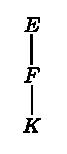
\includegraphics[scale=2.5]{Figures/torre_de_campos.pdf}
        \end{center}
        \caption{Torre de Campos}
    \end{wrapfigure}

    \lipsum
\end{proof}

\begin{excer}
    Sea $E/F$ una extensión algebraica. Demuestre que si $[E:F]=2$, entonces $E/F$ es extensión normal.
\end{excer}

\begin{proof}
    
\end{proof}

\begin{excer}
    Sean $E/F$ una extensión normal, $f(X)$ un polinomio con coeficientes en $F$ el cual es irredicible sobre $F[X]$. Sean $g(X)$ y $h(X)$ polinomios mónicos con coeficientes en $E$ irreducibles sobre $E[X]$ los cuales son factores de $f(X)$. Pruebe que existe un $F$-automorfismo de $E$ tal que $g^\phi(X)=h(X)$.
\end{excer}

\begin{proof}
    
\end{proof}

\begin{excer}
    Sea $E/F$ extensión algebraica. Demuestre que la extensión $E/F$ es normal si, y sólo si para cada polinomio irreducible $f(X)\in F[X]$, los factores irreducibles de $f(X)$ en $E[X]$ tienen el mismo grado.
\end{excer}

\begin{proof}
    
\end{proof}

\end{document}